% chktex-file 2% chktex-file 29
% chktex-file 13
\documentclass{report}
\usepackage{setspace}
\usepackage[a4paper, total={7in, 10in}]{geometry}
\usepackage[fleqn]{amsmath}
\usepackage{empheq}
\usepackage{amssymb}
\usepackage{amsthm}
\usepackage{gensymb}
\usepackage[fleqn]{cases}
\usepackage{multicol}
\usepackage{color}
\usepackage{stix}
\usepackage{chngcntr}
\usepackage{tikz}
\usepackage{enumitem}
\usepackage{pgfplots}
\usepackage{etoolbox}
\usepackage{tikz-3dplot}
\usepackage{tkz-euclide}
\usepackage{graphicx}
\usepackage{enumitem}
\usepackage{multirow}
\usepackage{mathtools}
\usepackage{mdframed}
\usepackage{adjustbox}

\def\nswe#1#2#3{#1\,$#2^\circ\,#3'$}
\graphicspath{ {./assets/} }
\usetikzlibrary{calc,trees,positioning,arrows,fit,shapes,calc, decorations.markings}
\newcommand{\midarrow}{\tikz \draw[-triangle 90] (0,0) -- +(.1,0);}

\newcommand\typel[2]{
  \mathbin{\mathop{#1\kern0pt}%
    \limits_{\raisebox{3.6ex}{\hbox to0pt{\hss\strut$\uparrow$\hss}}\hbox to0pt{\hss#2\hss}}}
}

\newcommand\typem[2]{
  \mathbin{\mathop{#1\kern0pt}%
    \limits^{\raisebox{3.6ex}{\hbox to0pt{\hss#2\hss}}\hbox to0pt{\hss\strut$\downarrow$\hss}}}
}

\counterwithout{equation}{chapter}
\setlength{\columnseprule}{1pt}
\setlength{\columnsep}{24pt}
\setcounter{chapter}{21}
\hfuzz=100pt

\newcommand{\pgfplotsdrawaxis}{\pgfplots@draw@axis}
\newcommand\perm[2][^n]{\prescript{#1\mkern-2.5mu}{}P_{#2}}
\newcommand\permtwo[2][^n]{{}_{#1}P_{#2}}
\newcommand\comb[2][^n]{{}_{#1}C_{#2}}
\newcommand\combtwo[2][^n]{\prescript{#1\mkern-2.5mu}{}C_{#2}}
\makeatother
\pgfplotsset{only axis on top/.style={axis on top=false, after end axis/.code={
          \pgfplotsset{axis line style=opaque, ticklabel style=opaque, tick style={thick,opaque},
            grid=none}\pgfplotsdrawaxis}}}

\newtheorem{theorem}{Theorem}

\mdfdefinestyle{MyFrame}{%
  linecolor=black,
  linewidth=1pt,
  roundcorner=20pt,
  innertopmargin=12pt, innerbottommargin=12pt, innerrightmargin=12pt,
  innerleftmargin=12pt, leftmargin = 4pt, rightmargin = 4pt, skipbelow=12pt,
  %backgroundcolor=gray!50!white}
}

\begin{document}
\newcommand{\sol}[1]{

  \noindent \textbf{Sol.}
}
\newcommand{\prooff}[1]{

  \noindent \textbf{Proof.}
}

\newenvironment{cequation}{
  \makeatletter
  \setbool{@fleqn}{false}
  \makeatother
  \begin{equation*}
    }{\end{equation*}}

\begin{titlepage}
  \raggedleft{}
  \rule{1pt}{\textheight}
  \hspace{0.02\textwidth}
  \parbox[b]{0.75\textwidth}{

  {\fontsize{40}{60}\selectfont\bfseries Mathematics}\\[2\baselineskip]
  {\huge\textit{Senior 3 Part I}}\\[4\baselineskip]
  {\Large\textsc{Melvin Chia}}

  \vspace{0.5\textheight}

  {\noindent Started on 10 April 2023}\\[\baselineskip]
  {\noindent Finished on XX XX 2023}\\[\baselineskip]
  {\noindent Actual time spent: XX days}\\[\baselineskip]}

\end{titlepage}

\chapter*{Introduction}
\addcontentsline{toc}{chapter}{Introduction} \markboth{INTRODUCTION}{}

\doublespacing{}
\section*{Why this book?}

\section*{Disclaimer}
\section*{Acknowledgements}

\singlespacing{}

\doublespacing{}
\tableofcontents
\singlespacing{}
\newpage

\begin{multicols}{2}
  \setstretch{1.25}

  \chapter{Function}

  \section{Definition of a Function}

  \subsection*{Mapping, Preimage and Image}

  For two non-empty sets $A$ and $B$, If an element $a$ inside set $A$ has a
  corresponding element $b$ inside set $B$, denoted as $a \to b$, then we say
  that $a$ is mapped to $b$ or $a$ and $b$ are paired. The mapping between two
  sets is normally denoted as $f$, $g$, $h$, etc. The mapping shown in the
  diagram below can be denoted as $f:1 \to x,\ 2 \to y,\ 4 \to z$.

  \begin{center}
    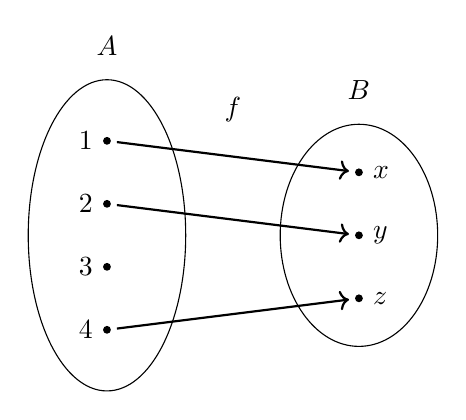
\begin{tikzpicture}[scale=0.8, ele/.style={fill=black,circle,minimum width=.8pt,inner sep=1pt},every fit/.style={ellipse,draw,inner sep=4pt}]
      \node[ele,label=left:$1$] (a1) at (0,4) {};
      \node[ele,label=left:$2$] (a2) at (0,3) {};
      \node[ele,label=left:$3$] (a3) at (0,2) {};
      \node[ele,label=left:$4$] (a4) at (0,1) {};

      \node[ele,,label=right:$z$] (b3) at (4,1.5) {};
      \node[ele,,label=right:$y$] (b2) at (4,2.5) {};
      \node[ele,,label=right:$x$] (b1) at (4,3.5) {};

      \node[draw,fit= (a1) (a2) (a3) (a4),minimum width=2cm] {} ;
      \node[draw,fit= (b1) (b2) (b3),minimum width=2cm] {} ;
      \draw[->,thick,shorten <=2pt,shorten >=2] (a1) -- (b1);
      \draw[->,thick,shorten <=2pt,shorten >=2] (a2) -- (b2);
      \draw[->,thick,shorten <=2pt,shorten >=2] (a4) -- (b3);
      \node at (2,4.5) {$f$};
      \node at (0,5.5) {$A$};
      \node at (4,4.8) {$B$};
    \end{tikzpicture}
  \end{center}

  Let $f:A \to B$ is a mapping, $a$ is an element in $A$. If $a$ is mapped to $b$
  under the mapping $f$, then $b$ is said to be the image of $a$ under the
  mapping $f$, denoted as $b = f(a)$; $a$ is said to be the preimage of $b$ under
  the mapping $f$. In the diagram above, under the mapping $f$, the image of $1$,
  $2$, and $4$ are $x$, $y$, and $z$ respectively, while the preimage of $x$,
  $y$, and $z$ are $1$, $2$, and $4$ respectively.

  \begin{mdframed}[style=MyFrame]
    Let $A$ and $B$ be two non-empty sets, $f$ is a mapping from $A$ to $B$ such that for all elements in $A$, there is a unique corresponding element in $B$, then $f$ is a function or a mapping from $A$ to $B$, denoted as $f:A \to B$.
  \end{mdframed}

  The mapping shown in the diagram below is a function.
  \begin{center}
    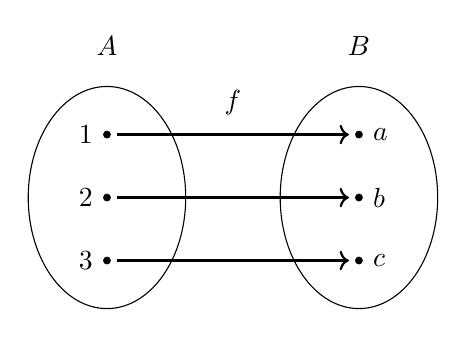
\begin{tikzpicture}[scale=0.8, ele/.style={fill=black,circle,minimum width=.8pt,inner sep=1pt},every fit/.style={ellipse,draw,inner sep=4pt}]
      \node[ele,label=left:$1$] (a1) at (0,4) {};
      \node[ele,label=left:$2$] (a2) at (0,3) {};
      \node[ele,label=left:$3$] (a3) at (0,2) {};

      \node[ele,,label=right:$c$] (b3) at (4,2) {};
      \node[ele,,label=right:$b$] (b2) at (4,3) {};
      \node[ele,,label=right:$a$] (b1) at (4,4) {};

      \node[draw,fit= (a1) (a2) (a3),minimum width=2cm] {} ;
      \node[draw,fit= (b1) (b2) (b3),minimum width=2cm] {} ;
      \draw[->,thick,shorten <=2pt,shorten >=2] (a1) -- (b1);
      \draw[->,thick,shorten <=2pt,shorten >=2] (a2) -- (b2);
      \draw[->,thick,shorten <=2pt,shorten >=2] (a3) -- (b3);
      \node at (2,4.5) {$f$};
      \node at (0,5.4) {$A$};
      \node at (4,5.4) {$B$};
    \end{tikzpicture}
  \end{center}

  \subsection{Practice 1}

  \begin{enumerate}
    \item For the following mappings, list the image of each element in $A$ and the
          preimage of each element in $B$, and determine whether the mapping is a
          function or not:
          \begin{enumerate}[]
            \item \adjustbox{valign=t}{
                    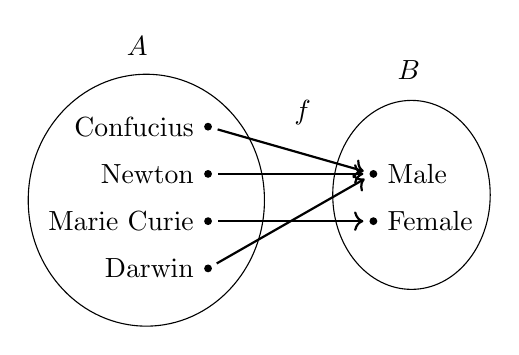
\begin{tikzpicture}[scale=0.6, ele/.style={fill=black,circle,minimum width=.8pt,inner sep=1pt},every fit/.style={ellipse,draw,inner sep=4pt}]
                      \node[ele,label=left:Confucius] (a1) at (0.5,4) {};
                      \node[ele,label=left:Newton] (a2) at (0.5,3) {};
                      \node[ele,label=left:Marie Curie] (a3) at (0.5,2) {};
                      \node[ele,label=left:Darwin] (a4) at (0.5,1) {};
                      \node[label=left:] (a999) at (-2,1) {};

                      \node[ele,,label=right:Female] (b2) at (4,2) {};
                      \node[ele,,label=right:Male] (b1) at (4,3) {};
                      \node[] (b999) at (5.5,3) {};

                      \node[draw,fit= (a1) (a2) (a3) (a4) (a999),minimum width=3cm] {} ;
                      \node[draw,fit= (b1) (b2) (b999),minimum width=2cm, minimum height=2.4cm] {} ;
                      \draw[->,thick,shorten <=2pt,shorten >=2] (a1) -- (b1);
                      \draw[->,thick,shorten <=2pt,shorten >=2] (a2) -- (b1);
                      \draw[->,thick,shorten <=2pt,shorten >=2] (a3) -- (b2);
                      \draw[->,thick,shorten <=2pt,shorten >=2] (a4) -- (b1);
                      \node at (2.5,4.3) {$f$};
                      \node at (-1,5.7) {$A$};
                      \node at (4.75,5.2) {$B$};
                    \end{tikzpicture}
                  }

            \item \adjustbox{valign=t}{
                    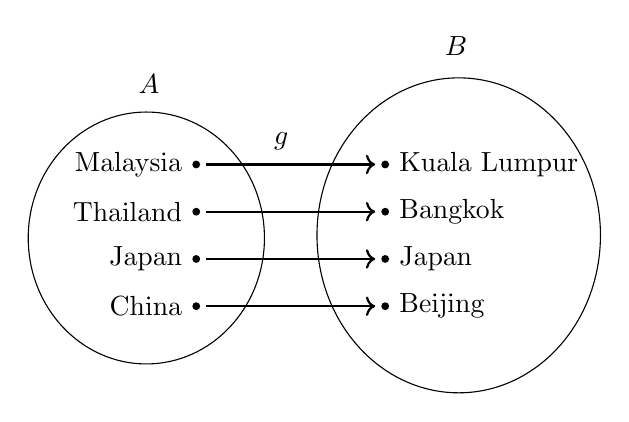
\begin{tikzpicture}[scale=0.6, ele/.style={fill=black,circle,minimum width=.8pt,inner sep=1pt},every fit/.style={ellipse,draw,inner sep=4pt}]
                      \node[ele,label=left:Malaysia] (a1) at (0,4) {};
                      \node[ele,label=left:Thailand] (a2) at (0,3) {};
                      \node[ele,label=left:Japan] (a3) at (0,2) {};
                      \node[ele,label=left:China] (a4) at (0,1) {};
                      \node[label=left:] (a999) at (-2,1) {};

                      \node[ele,,label=right:Kuala Lumpur] (b1) at (4,4) {};
                      \node[ele,,label=right:Bangkok] (b2) at (4,3) {};
                      \node[ele,,label=right:Japan] (b3) at (4,2) {};
                      \node[ele,,label=right:Beijing] (b4) at (4,1) {};
                      \node[] (b999) at (7,3) {};

                      \node[draw,fit= (a1) (a2) (a3) (a4) (a999),minimum width=3cm] {} ;
                      \node[draw,fit= (b1) (b2) (b3) (b4) (b999),minimum width=3.6cm, minimum height=4cm] {} ;
                      \draw[->,thick,shorten <=2pt,shorten >=2] (a1) -- (b1);
                      \draw[->,thick,shorten <=2pt,shorten >=2] (a2) -- (b2);
                      \draw[->,thick,shorten <=2pt,shorten >=2] (a3) -- (b3);
                      \draw[->,thick,shorten <=2pt,shorten >=2] (a4) -- (b4);
                      \node at (1.8,4.5) {$g$};
                      \node at (-1,5.7) {$A$};
                      \node at (5.5,6.5) {$B$};
                    \end{tikzpicture}
                  }

            \item \adjustbox{valign=t}{
                    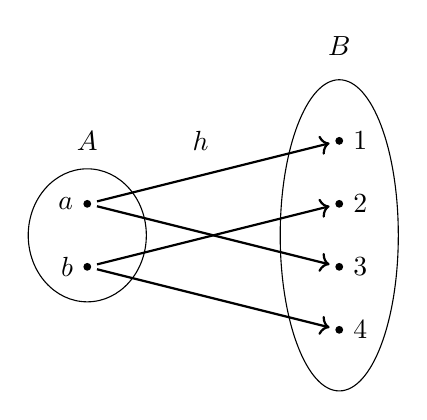
\begin{tikzpicture}[scale=0.8, ele/.style={fill=black,circle,minimum width=.8pt,inner sep=1pt},every fit/.style={ellipse,draw,inner sep=4pt}]
                      \node[ele,label=left:$a$] (a1) at (0,3) {};
                      \node[ele,label=left:$b$] (a2) at (0,2) {};

                      \node[ele,,label=right:$1$] (b1) at (4,4) {};
                      \node[ele,,label=right:$2$] (b2) at (4,3) {};
                      \node[ele,,label=right:$3$] (b3) at (4,2) {};
                      \node[ele,,label=right:$4$] (b4) at (4,1) {};

                      \node[draw,fit= (a1) (a2),minimum width=1.5cm] {} ;
                      \node[draw,fit= (b1) (b2) (b3) (b4),minimum width=1.5cm] {} ;
                      \draw[->,thick,shorten <=2pt,shorten >=2] (a1) -- (b1);
                      \draw[->,thick,shorten <=2pt,shorten >=2] (a2) -- (b2);
                      \draw[->,thick,shorten <=2pt,shorten >=2] (a1) -- (b3);
                      \draw[->,thick,shorten <=2pt,shorten >=2] (a2) -- (b4);
                      \node at (1.8,4) {$h$};
                      \node at (0,4) {$A$};
                      \node at (4,5.5) {$B$};
                    \end{tikzpicture}
                  }

            \item \adjustbox{valign=t}{
                    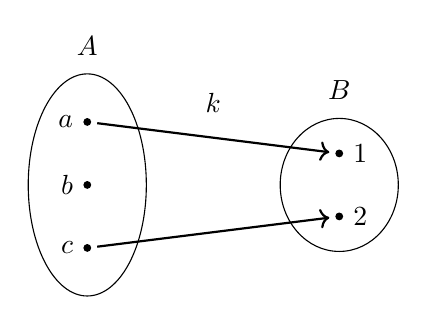
\begin{tikzpicture}[scale=0.8, ele/.style={fill=black,circle,minimum width=.8pt,inner sep=1pt},every fit/.style={ellipse,draw,inner sep=4pt}]
                      \node[ele,label=left:$a$] (a1) at (0,3) {};
                      \node[ele,label=left:$b$] (a2) at (0,2) {};
                      \node[ele,label=left:$c$] (a3) at (0,1) {};

                      \node[ele,,label=right:$1$] (b1) at (4,2.5) {};
                      \node[ele,,label=right:$2$] (b2) at (4,1.5) {};

                      \node[draw,fit= (a1) (a2) (a3),minimum width=1.5cm] {} ;
                      \node[draw,fit= (b1) (b2),minimum width=1.5cm] {} ;
                      \draw[->,thick,shorten <=2pt,shorten >=2] (a1) -- (b1);
                      \draw[->,thick,shorten <=2pt,shorten >=2] (a3) -- (b2);
                      \node at (2,3.3) {$k$};
                      \node at (0,4.2) {$A$};
                      \node at (4,3.5) {$B$};
                    \end{tikzpicture}
                  }
          \end{enumerate}

    \item Given a mapping $g:x \to x+3$, $x \in\big\{$-2, -1, 0, 1, 2, 3$\big\}$, find
          the image of each $x$.

    \item Determine whether the following mappings are functions.
          \begin{enumerate}
            \item \adjustbox{valign=t}{
                    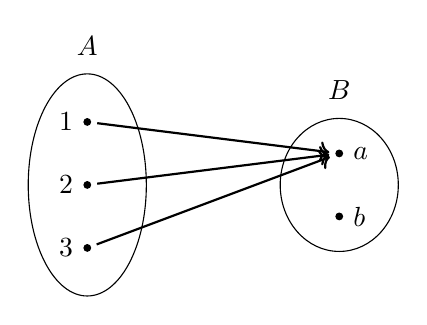
\begin{tikzpicture}[scale=0.8, ele/.style={fill=black,circle,minimum width=.8pt,inner sep=1pt},every fit/.style={ellipse,draw,inner sep=4pt}]
                      \node[ele,label=left:$1$] (a1) at (0,3) {};
                      \node[ele,label=left:$2$] (a2) at (0,2) {};
                      \node[ele,label=left:$3$] (a3) at (0,1) {};

                      \node[ele,,label=right:$a$] (b1) at (4,2.5) {};
                      \node[ele,,label=right:$b$] (b2) at (4,1.5) {};

                      \node[draw,fit= (a1) (a2) (a3),minimum width=1.5cm] {} ;
                      \node[draw,fit= (b1) (b2),minimum width=1.5cm] {} ;
                      \draw[->,thick,shorten <=2pt,shorten >=2] (a1) -- (b1);
                      \draw[->,thick,shorten <=2pt,shorten >=2] (a2) -- (b1);
                      \draw[->,thick,shorten <=2pt,shorten >=2] (a3) -- (b1);
                      \node at (0,4.2) {$A$};
                      \node at (4,3.5) {$B$};
                    \end{tikzpicture}
                  }

            \item \adjustbox{valign=t}{
                    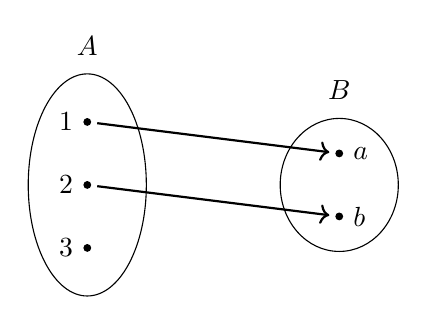
\begin{tikzpicture}[scale=0.8, ele/.style={fill=black,circle,minimum width=.8pt,inner sep=1pt},every fit/.style={ellipse,draw,inner sep=4pt}]
                      \node[ele,label=left:$1$] (a1) at (0,3) {};
                      \node[ele,label=left:$2$] (a2) at (0,2) {};
                      \node[ele,label=left:$3$] (a3) at (0,1) {};

                      \node[ele,,label=right:$a$] (b1) at (4,2.5) {};
                      \node[ele,,label=right:$b$] (b2) at (4,1.5) {};

                      \node[draw,fit= (a1) (a2) (a3),minimum width=1.5cm] {} ;
                      \node[draw,fit= (b1) (b2),minimum width=1.5cm] {} ;
                      \draw[->,thick,shorten <=2pt,shorten >=2] (a1) -- (b1);
                      \draw[->,thick,shorten <=2pt,shorten >=2] (a2) -- (b2);
                      \node at (0,4.2) {$A$};
                      \node at (4,3.5) {$B$};
                    \end{tikzpicture}
                  }

            \item \adjustbox{valign=t}{
                    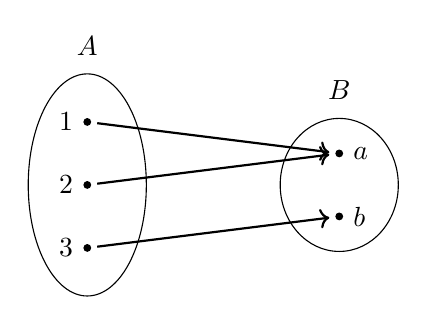
\begin{tikzpicture}[scale=0.8, ele/.style={fill=black,circle,minimum width=.8pt,inner sep=1pt},every fit/.style={ellipse,draw,inner sep=4pt}]
                      \node[ele,label=left:$1$] (a1) at (0,3) {};
                      \node[ele,label=left:$2$] (a2) at (0,2) {};
                      \node[ele,label=left:$3$] (a3) at (0,1) {};

                      \node[ele,,label=right:$a$] (b1) at (4,2.5) {};
                      \node[ele,,label=right:$b$] (b2) at (4,1.5) {};

                      \node[draw,fit= (a1) (a2) (a3),minimum width=1.5cm] {} ;
                      \node[draw,fit= (b1) (b2),minimum width=1.5cm] {} ;
                      \draw[->,thick,shorten <=2pt,shorten >=2] (a1) -- (b1);
                      \draw[->,thick,shorten <=2pt,shorten >=2] (a2) -- (b1);
                      \draw[->,thick,shorten <=2pt,shorten >=2] (a3) -- (b2);
                      \node at (0,4.2) {$A$};
                      \node at (4,3.5) {$B$};
                    \end{tikzpicture}
                  }

            \item \adjustbox{valign=t}{
                    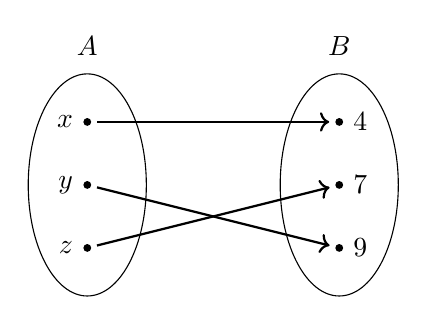
\begin{tikzpicture}[scale=0.8, ele/.style={fill=black,circle,minimum width=.8pt,inner sep=1pt},every fit/.style={ellipse,draw,inner sep=4pt}]
                      \node[ele,label=left:$x$] (a1) at (0,3) {};
                      \node[ele,label=left:$y$] (a2) at (0,2) {};
                      \node[ele,label=left:$z$] (a3) at (0,1) {};

                      \node[ele,,label=right:$4$] (b1) at (4,3) {};
                      \node[ele,,label=right:$7$] (b2) at (4,2) {};
                      \node[ele,,label=right:$9$] (b3) at (4,1) {};

                      \node[draw,fit= (a1) (a2) (a3),minimum width=1.5cm] {} ;
                      \node[draw,fit= (b1) (b2) (b3),minimum width=1.5cm] {} ;
                      \draw[->,thick,shorten <=2pt,shorten >=2] (a1) -- (b1);
                      \draw[->,thick,shorten <=2pt,shorten >=2] (a2) -- (b3);
                      \draw[->,thick,shorten <=2pt,shorten >=2] (a3) -- (b2);
                      \node at (0,4.2) {$A$};
                      \node at (4,4.2) {$B$};
                    \end{tikzpicture}
                  }

            \item \adjustbox{valign=t}{
                    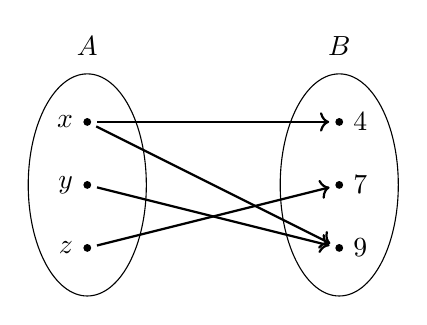
\begin{tikzpicture}[scale=0.8, ele/.style={fill=black,circle,minimum width=.8pt,inner sep=1pt},every fit/.style={ellipse,draw,inner sep=4pt}]
                      \node[ele,label=left:$x$] (a1) at (0,3) {};
                      \node[ele,label=left:$y$] (a2) at (0,2) {};
                      \node[ele,label=left:$z$] (a3) at (0,1) {};

                      \node[ele,,label=right:$4$] (b1) at (4,3) {};
                      \node[ele,,label=right:$7$] (b2) at (4,2) {};
                      \node[ele,,label=right:$9$] (b3) at (4,1) {};

                      \node[draw,fit= (a1) (a2) (a3),minimum width=1.5cm] {} ;
                      \node[draw,fit= (b1) (b2) (b3),minimum width=1.5cm] {} ;
                      \draw[->,thick,shorten <=2pt,shorten >=2] (a1) -- (b1);
                      \draw[->,thick,shorten <=2pt,shorten >=2] (a1) -- (b3);
                      \draw[->,thick,shorten <=2pt,shorten >=2] (a2) -- (b3);
                      \draw[->,thick,shorten <=2pt,shorten >=2] (a3) -- (b2);
                      \node at (0,4.2) {$A$};
                      \node at (4,4.2) {$B$};
                    \end{tikzpicture}
                  }

            \item \adjustbox{valign=t}{
                    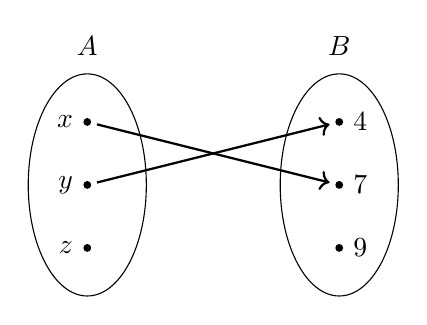
\begin{tikzpicture}[scale=0.8, ele/.style={fill=black,circle,minimum width=.8pt,inner sep=1pt},every fit/.style={ellipse,draw,inner sep=4pt}]
                      \node[ele,label=left:$x$] (a1) at (0,3) {};
                      \node[ele,label=left:$y$] (a2) at (0,2) {};
                      \node[ele,label=left:$z$] (a3) at (0,1) {};

                      \node[ele,,label=right:$4$] (b1) at (4,3) {};
                      \node[ele,,label=right:$7$] (b2) at (4,2) {};
                      \node[ele,,label=right:$9$] (b3) at (4,1) {};

                      \node[draw,fit= (a1) (a2) (a3),minimum width=1.5cm] {} ;
                      \node[draw,fit= (b1) (b2) (b3),minimum width=1.5cm] {} ;
                      \draw[->,thick,shorten <=2pt,shorten >=2] (a1) -- (b2);
                      \draw[->,thick,shorten <=2pt,shorten >=2] (a2) -- (b1);
                      \node at (0,4.2) {$A$};
                      \node at (4,4.2) {$B$};
                    \end{tikzpicture}
                  }
          \end{enumerate}
  \end{enumerate}

  The function $f: A \to B$ can be written as $y = f(x)$, $x$ is the element of
  $A$ and $y$ is the element of $B$. When $x$ changes, $y$ changes as well. $x$
  is called independent variable, while $y$ is called dependent variable.

  Keep in mind that $f(x)$ is NOT the product of $f$ and $x$.

  \subsection*{Representation of Functions}

  Generally speaking, there are a few ways to represent a function:
  \begin{enumerate}
    \item \textbf{Narrative Form}: express the function of two sets in words. For example, Let $A = \big\{1, 2, 3\big\}$ and $B = \big\{1, 4, 9\big\}$, $f$ is a function from $A$ to $B$, its definition is that for any element $x$ in $A$, its corresponding element is $x^2$ in $B$.
    \item \textbf{Arrow Method}: draw an arrow to connect the preimage and image of a function such that the preimage is corresponding to the image. To express the example above, we express it as $f: 1 \to 1,\ 2 \to 4,\ 3 \to 9$.
    \item \textbf{Analytical Method}: express the function in the form of mathematical expression to represent the relationship between the independent variable and the dependent variable. For example, $f(x) = x^2, x \in \mathbb{A}$.
    \item \textbf{Venn Diagram}: draw arrows between the venn diagram of two sets to represent the function, as shown below:
          \begin{center}
            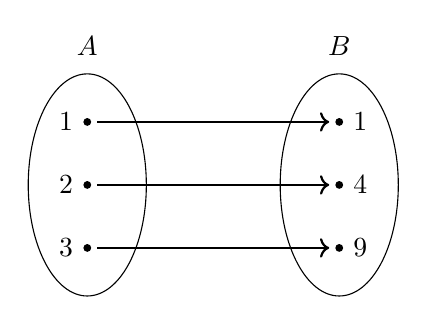
\begin{tikzpicture}[scale=0.8, ele/.style={fill=black,circle,minimum width=.8pt,inner sep=1pt},every fit/.style={ellipse,draw,inner sep=4pt}]
              \node[ele,label=left:$1$] (a1) at (0,3) {};
              \node[ele,label=left:$2$] (a2) at (0,2) {};
              \node[ele,label=left:$3$] (a3) at (0,1) {};

              \node[ele,,label=right:$1$] (b1) at (4,3) {};
              \node[ele,,label=right:$4$] (b2) at (4,2) {};
              \node[ele,,label=right:$9$] (b3) at (4,1) {};

              \node[draw,fit= (a1) (a2) (a3),minimum width=1.5cm] {} ;
              \node[draw,fit= (b1) (b2) (b3),minimum width=1.5cm] {} ;
              \draw[->,thick,shorten <=2pt,shorten >=2] (a1) -- (b1);
              \draw[->,thick,shorten <=2pt,shorten >=2] (a2) -- (b2);
              \draw[->,thick,shorten <=2pt,shorten >=2] (a3) -- (b3);
              \node at (0,4.2) {$A$};
              \node at (4,4.2) {$B$};
            \end{tikzpicture}
          \end{center}
    \item \textbf{Table Method}: express the function in the form of table, showing the relationship of the chosen value between independent variable $x$ and the value of its corresponding dependent variable $y$, as shown below:
          \begin{center}
            \begin{tabular}{|c|c|c|c|}
              \hline
              $x$ & $1$ & $2$ & $3$ \\
              \hline
              $y$ & $1$ & $4$ & $9$ \\
              \hline
            \end{tabular}
          \end{center}

    \item \textbf{Graphical Method}: draw a graph to represent the function of the two variables, as shown below:
          \begin{center}
            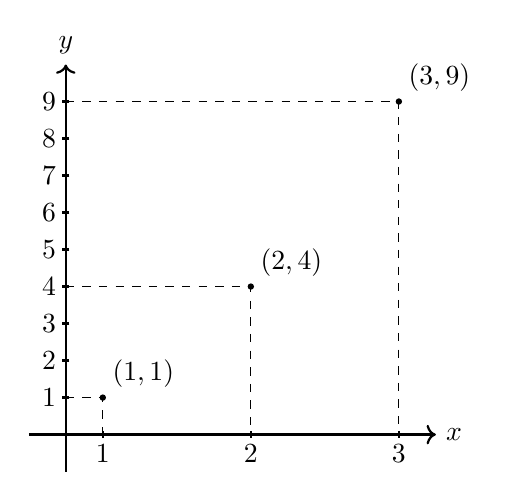
\begin{tikzpicture}[scale=0.47]
              \draw[->,thick] (-1,0) -- (10,0) node[right] {$x$};
              \draw[->,thick] (0,-1) -- (0,10) node[above] {$y$};
              \draw[thick] (1,0.1) -- (1,-0.1);
              \node[below] at (1,0) {1};
              \draw[thick] (5,0.1) -- (5,-0.1);
              \node[below] at (5,0) {2};
              \draw[thick] (9,0.1) -- (9,-0.1);
              \node[below] at (9,0) {3};
              \foreach \y in {1,...,9}
                {
                  \draw[thick] (0.1,\y) -- (-0.1,\y);
                  \node[left] at (0,\y) {\y};
                }
              \filldraw (1, 1) circle (2pt) node[above right]{$(1,1)$};
              \filldraw (5, 4) circle (2pt) node[above right]{$(2,4)$};
              \filldraw (9, 9) circle (2pt) node[above right]{$(3,9)$};
              \draw[dashed] (0,1) -- (1,1) -- (1,0);
              \draw[dashed] (0,4) -- (5,4) -- (5,0);
              \draw[dashed] (0,9) -- (9,9) -- (9,0);
            \end{tikzpicture}
          \end{center}
  \end{enumerate}

  \subsection{Practice 2}

  Express the following functions using analytical method, venn diagram, table
  method and graphical method.
  \begin{enumerate}[label=(\alph*)]
    \item $f$ mapping each integers from $-3$ to $3$ to its squares plus $4$.
    \item $g$ mapping each natural numbers from $1$ to $4$ to its cubes.
  \end{enumerate}

  \subsection{Exercise 22.1}

  \begin{enumerate}
    \item Express the mapping from set $A$ to set $B$, and determine which of the
          following mappings are functions.

          \resizebox{22em}{!}{
            \begin{tabular}{|c|c|c|c|}
              \hline
                  & Set $A$                                & Set $B$                                                                   & Mapping       \\
              \hline
              (a) & \{0, 3, 9, 12\}                        & \{0, 1, 2, 3\}                                                            & Divide by $3$ \\
              \hline
              (b) & \{-2, -1, 0, 1, 2\}                    & \{0, 1, 4, 9, 16\}                                                        & Power of $4$  \\
              \hline
              (c) & \{-2, -1, 0, 1, 2\}                    & \{0, 1, 4\}                                                               & Square        \\
              \hline
              (d) & \{30$^\circ$, 45$^\circ$, 60$^\circ$\} & $\left\{\dfrac{1}{2},\ \dfrac{\sqrt{2}}{2},\ \dfrac{\sqrt{3}}{2}\right\}$ & Sine          \\
              \hline
              (e) & \{-1, 0, 1, 2\}                        & \{-1, 0, 1\}                                                              & Cube          \\
              \hline
            \end{tabular}
          }

    \item Let function $f(x) = 3x^2 + 1$.
          \begin{enumerate}
            \item Find the image of the following elements:
                  \begin{enumerate}
                    \item -3
                    \item -2
                    \item 0
                    \item 2
                    \item 5
                  \end{enumerate}
            \item Find the preimage of the following elements:
                  \begin{enumerate}
                    \item 13
                    \item 28
                    \item 1
                    \item 0
                    \item 4
                  \end{enumerate}
          \end{enumerate}

    \item Let function $g(x) = 5x-2$. Find:
          \begin{enumerate}
            \item $g(-2)$
            \item $g(-1)$
            \item $g(0)$
          \end{enumerate}

    \item Let function $f(x) = \left\{\begin{array}{ll}
              \ \ \ \ \ \ 2x, & x \leq -1     \\
              \ \ x-1,        & -1 \leq x < 3 \\
              4x + 2,         & x \geq 3
            \end{array}\right.$, find

          \begin{enumerate}
            \item $f(-5)$
            \item $f(-2)$
            \item $f(0)$
            \item $f(2)$
            \item $f(10)$
          \end{enumerate}

    \item Let $f: \mathbb{R} \to \mathbb{R}$, $f(x) = x^4$. Find the image of $-1$, 0, 1,
          and 2 under $f$.

    \item Let $f: \mathbb{R} \to \mathbb{R}$, $f(x) = x^4$. Find the preimage of 0, 1,
          and 4 under $f$.

          In $\mathbb{R}$, which element does not have a preimage?

    \item In the diagram below, given that function $g: A \to B$ is defined as $g: x \to
            2x - 8$. Find the value of $a$ and $b$.
          \begin{center}
            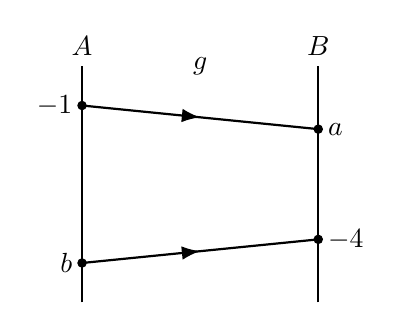
\begin{tikzpicture}
              \draw[thick] (0,0) -- (0,3) node[above]{$A$};
              \draw[thick] (3,0) -- (3,3) node[above]{$B$};
              \node at (1.5, 3) {$g$};
              \filldraw (0, 2.5) circle (1.5pt) node[left]{$-1$};
              \filldraw (0, 0.5) circle (1.5pt) node[left]{$b$};
              \filldraw (3, 0.8) circle (1.5pt) node[right]{$-4$};
              \filldraw (3, 2.2) circle (1.5pt) node[right]{$a$};
              \begin{scope}[thick,decoration={
                      markings,
                      mark=at position 0.5 with {\arrow{Latex}}}
                ]
                \draw[postaction={decorate}] (0, 2.5) -- (3, 2.2);
                \draw[postaction={decorate}] (0, 0.5) -- (3, 0.8);
              \end{scope}
            \end{tikzpicture}
          \end{center}

    \item Using narrative form, arrow method, venn diagram, table method and graphical
          method, express the function $f(x) = 2x$, $x \in \{-2, -1, 0, 1, 2\}$.
  \end{enumerate}

  \section{Domain and Range}

  \begin{mdframed}[style=MyFrame]
    Let $f$ is a function from set $A$ to set $B$, then set $A$ is called the domain of $f$, denoted by $D_f$; set $B$ is called the codomain of $f$; the set of the images of all elements of $A$ under $f$ is called the range of $f$, denoted by $R_f$.
  \end{mdframed}

  If the domain $A$ and range $B$ of function $f: A\to B$ are both subsets of
  real number set $\mathbb{R}$, then this function is called real valued function
  / real function. This book primarily discusses about real valued functions.
  When the domain of a real function is not mentioned and only the mapping rule
  is given, its domain is assumed to be the set of all real numbers that yield
  defined values $f(x)$. After the domain and the mapping rule are determined,
  the range of a function will then be determined.

  \begin{center}
    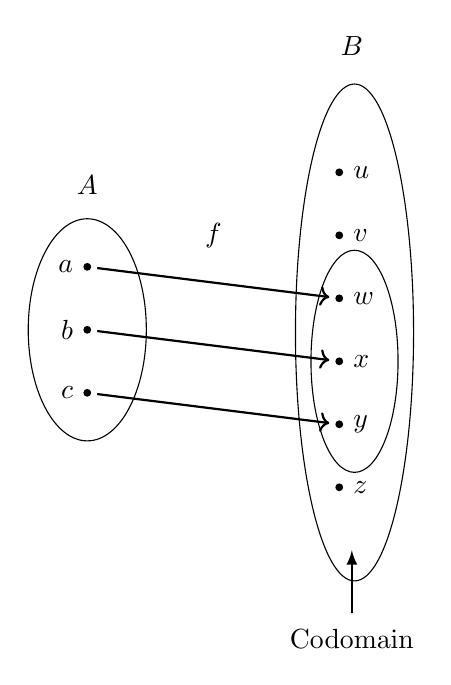
\begin{tikzpicture}[scale=0.8, ele/.style={fill=black,circle,minimum width=.8pt,inner sep=1pt},every fit/.style={ellipse,draw,inner sep=4pt}]
      \node[ele,label=left:$a$] (a1) at (0,4.5) {};
      \node[ele,label=left:$b$] (a2) at (0,3.5) {};
      \node[ele,label=left:$c$] (a3) at (0,2.5) {};

      \node[ele,,label=right:$u$] (b1) at (4,6) {};
      \node[ele,,label=right:$v$] (b2) at (4,5) {};
      \node[ele,,label=right:$w$] (b3) at (4,4) {};
      \node[ele,,label=right:$x$] (b4) at (4,3) {};
      \node[ele,,label=right:$y$] (b5) at (4,2) {};
      \node[ele,,label=right:$z$] (b6) at (4,1) {};
      \node[] (b999) at (4.4,1) {};
      \node[] (b998) at (4.4,3) {};

      \node[draw,fit= (a1) (a2) (a3),minimum width=1.5cm] {} ;
      \node[draw,fit= (b1) (b2) (b3) (b4) (b5) (b6) (b999),minimum width=1.5cm] {} ;
      \node[draw,fit= (b3) (b4) (b5) (b998),minimum width=1cm] {} ;
      \draw[->,thick,shorten <=2pt,shorten >=2] (a1) -- (b3);
      \draw[->,thick,shorten <=2pt,shorten >=2] (a2) -- (b4);
      \draw[->,thick,shorten <=2pt,shorten >=2] (a3) -- (b5);
      \node at (0,5.8) {$A$};
      \node at (4.2,8) {$B$};
      \node at (2,5) {$f$};
      \draw[thick, -latex](4.2,-1) -- (4.2,0);
      \node at (4.2,-1.4) {Codomain};
    \end{tikzpicture}
  \end{center}

  \section{Graphs of Functions and Their Transformations}

  \section{Composite Functions}

  \section{One to One Function, Onto Function and One to One Onto Function}

  \section{Inverse Functions}

  \chapter{Exponents and Logarithms}

  \section{Exponents}

  \section{Logarithms}

  \section{Arithmetic Properties of Logarithms and Base Changing Formula}

  \section{Exponential Equations}

  \section{Logarithmic Equations}

  \section{Compound Interest and Annuity}

  \chapter{Limits}

  \section{Concept of Limits}

  \section{Limits of Functions}

  \section{Arithmetic Properties of Limits of Functions}

  \chapter{Differentiation}

  \section{Gradient of Tangent Line on a Curve}

  \section{Gradient of Tangent Line and Derivative}

  \section{Law of Differentiation}

  \section{Chain Rule - Differentiation of Composite Functions}

  \section{Higher Order Derivatives}

  \section{Implicit Differentiation}

  \section{Two Basic Limits}

  \section{Derivatives of Trigonometric Functions}

  \section{Derivatives of Exponential Functions}

  \section{Derivatives of Logarithmic Functions}

\end{multicols}

\end{document}